\documentclass[journal]{vgtc}       % preprint (journal style)

%% Uncomment one of the lines above depending on where your paper is
%% in the conference process. ``review'' and ``widereview'' are for review
%% submission, ``preprint'' is for pre-publication, and the final version
%% doesn't use a specific qualifier. Further, ``electronic'' includes
%% hyperreferences for more convenient online viewing.

%% Please use one of the ``review'' options in combination with the
%% assigned online id (see below) ONLY if your paper uses a double blind
%% review process. Some conferences, like IEEE Vis and InfoVis, have NOT
%% in the past.

%% Please note that the use of figures other than the optional teaser is not permitted on the first page
%% of the journal version.  Figures should begin on the second page and be
%% in CMYK or Grey scale format, otherwise, colour shifting may occur
%% during the printing process.  Papers submitted with figures other than the optional teaser on the
%% first page will be refused.

%% These three lines bring in essential packages: ``mathptmx'' for Type 1
%% typefaces, ``graphicx'' for inclusion of EPS figures. and ``times''
%% for proper handling of the times font family.

\usepackage{mathptmx}
\usepackage{graphicx}
\usepackage{times}
\usepackage{caption}
\usepackage{color}
\usepackage{bm}
\usepackage{amsmath}
\usepackage{microtype}
\usepackage[normalem]{ulem}

% options for TODO: either use red bold font for litle annotations (which do not work very well)

%\newcommand{\todo}[1]{\textcolor{red}{\textbf{TODO:} #1}}

% following commands are 'non standard' and not bundled with template, delete it problems occur
\usepackage{xargs}                      % Use more than one optional parameter in a new commands
\usepackage[pdftex,dvipsnames]{xcolor}  % Coloured text etc.
\usepackage[colorinlistoftodos,prependcaption,textsize=tiny]{todonotes}
\newcommand{\unsure}[1]{\todo[linecolor=red,backgroundcolor=red!25,bordercolor=red,inline]{#1}}
\newcommand{\change}[1]{\todo[linecolor=blue,backgroundcolor=blue!25,bordercolor=blue,inline]{#1}}
\newcommand{\info}[1]{\todo[linecolor=OliveGreen,backgroundcolor=OliveGreen!25,bordercolor=OliveGreen,inline]{#1}}
\newcommand{\improvement}[1]{\todo[linecolor=Plum,backgroundcolor=Plum!25,bordercolor=Plum,inline]{#1}}
\newcommand{\thiswillnotshow}[1]{\todo[disable,inline]{#1}}



\captionsetup[table]{justification=justified,singlelinecheck=false}
\captionsetup[figure]{justification=justified,singlelinecheck=false}

%% We encourage the use of mathptmx for consistent usage of times font
%% throughout the proceedings. However, if you encounter conflicts
%% with other math-related packages, you may want to disable it.

%% allow for this line if you want the electronic option to work properly
\vgtcinsertpkg

%% Paper title.

\title{Comparative Visualization of Molecular Surfaces using Similarity-based Clustering}

%% This is how authors are specified in the journal style

%% indicate IEEE Member or Student Member in form indicated below
\author{Wilhelm Buchm\"uller, Shoma Kaiser, Damir Ravilija, Enis ...}
\authorfooter{
%% insert punctuation at end of each item
\begin{tabular}{cccc}
  Wilhelm Buchmüller  & Shoma Kaiser & Enis .. . & Damir Rwilja  \\
 buch.willi@googlemail.com     & example@example.com       & example@example.com & example@example.com
%% Warning: The final version of the paper will be published on the
%% web. If you don't want to see your private mail adress on the web,
%% use your studi address.
\end{tabular}
}

%other entries to be set up for journal
%\shortauthortitle{Schmid \MakeLowercase{\textit{et\,al.}}: ProjINF for fun and profit}

%% Abstract section.
\abstract{
Lorem ipsum dolor sit amet, consetetur sadipscing elitr, sed diam nonumy eirmod tempor invidunt ut labore et dolore magna aliquyam erat, sed diam voluptua. At vero eos et accusam et justo duo dolores et ea rebum. Stet clita kasd gubergren, no sea takimata sanctus est Lorem ipsum dolor sit amet. Lorem ipsum dolor sit amet, consetetur sadipscing elitr, sed diam nonumy eirmod tempor invidunt ut labore et dolore magna aliquyam erat, sed diam voluptua. At vero eos et accusam et justo duo dolores et ea rebum. Stet clita kasd gubergren, no sea takimata sanctus est Lorem ipsum dolor sit amet.
} % end of abstract

%% Keywords that describe your work. Will show as 'Index Terms' in journal
%% please capitalize first letter and insert punctuation after last keyword
\keywords{Visualization in Physical Sciences and Engineering, Glyph-based Techniques, Time-varying Data, Point-Based Data.}

%% ACM Computing Classification System (CCS).
%% See <http://www.acm.org/class/1998/> for details.
%% The ``\CCScat'' command takes four arguments.

\CCScatlist{ % not used in journal version
	\CCScat{Computer Graphics}{I.3.8}{Applications}{Molecular Dynamics Visualization}
	\CCScat{Simulation and Modeling}{I.6.6}{Simulation Output Analysis}{Molecular Dynamics Visualization}
	\CCScat{Computer Graphics}{I.3.7}{Three-Dimensional Graphics and Realism}{Raytracing}
}

\graphicspath{{pics/}}

%% Uncomment below to include a teaser figure.
%\teaser{
%\centering
%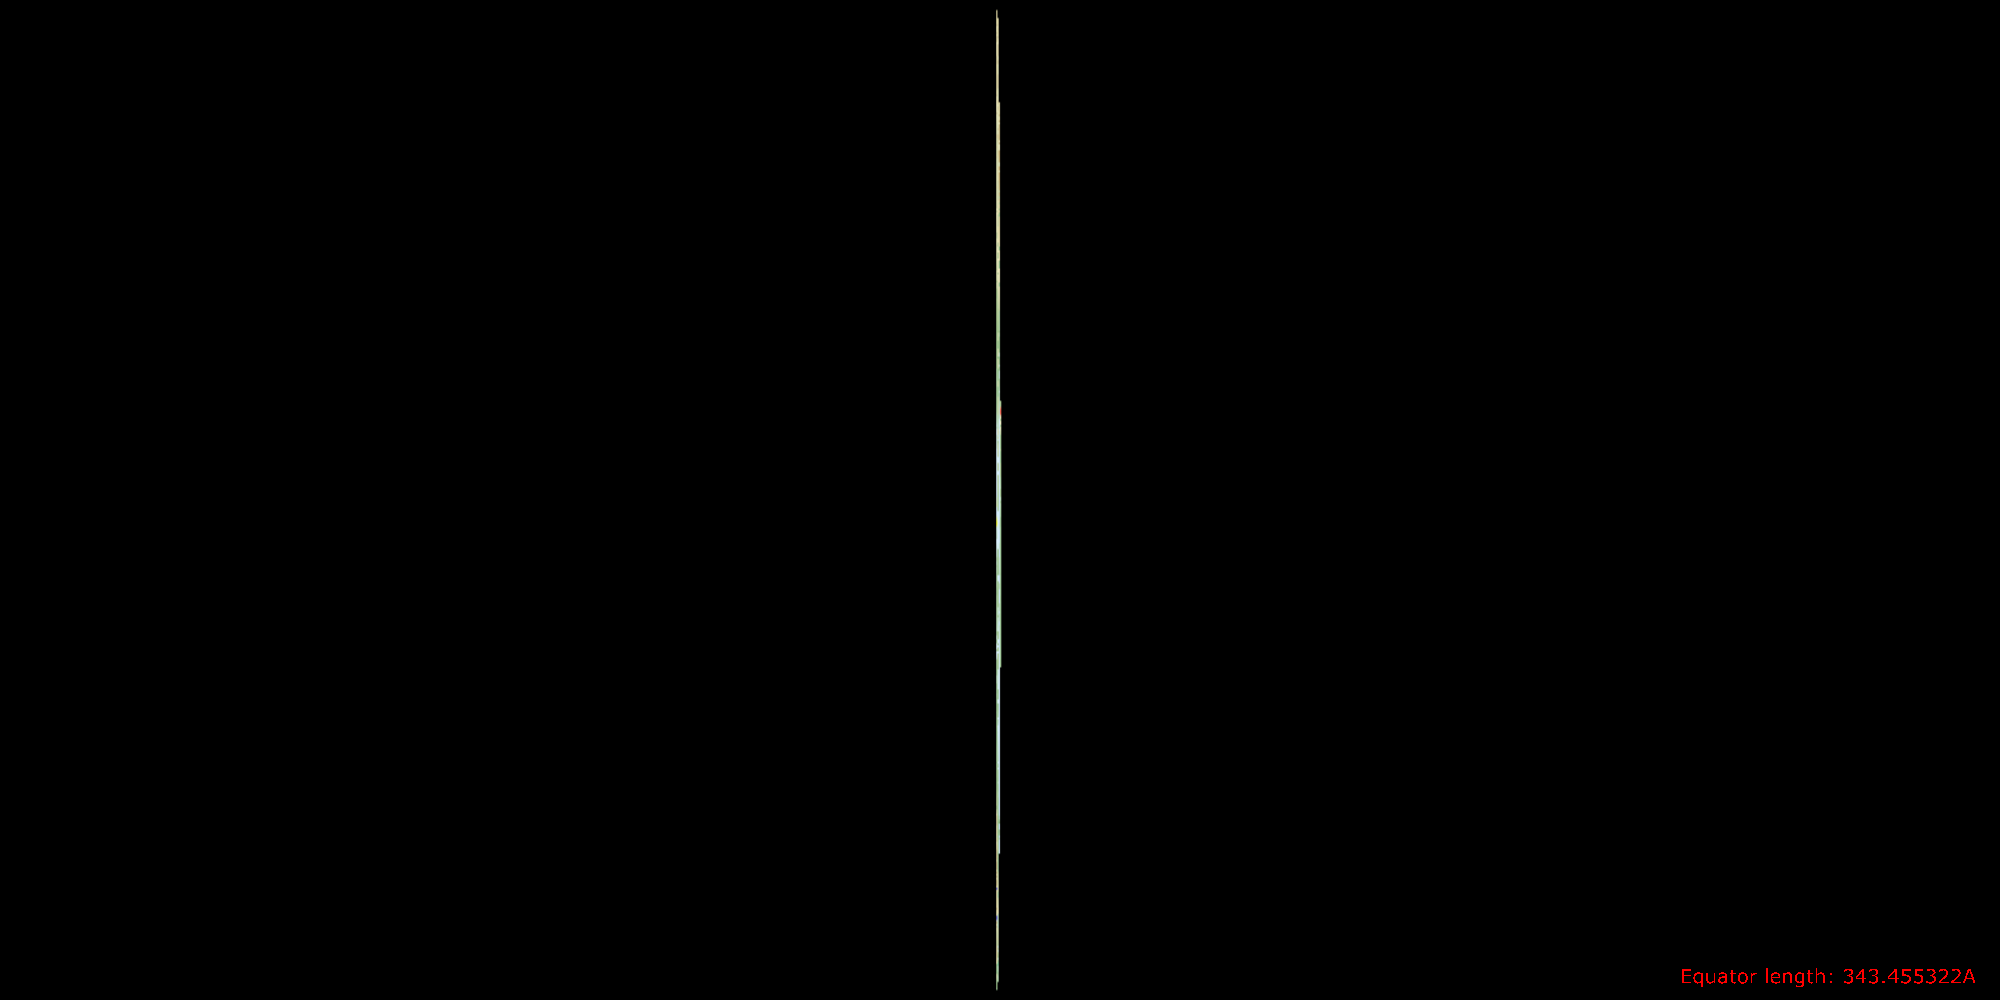
\includegraphics[width=12cm]{teaser}
%\caption{blah
%}\label{fig:teaser}
%}

%%%%%%%%%%%%%%%%%%%%%%%%%%%%%%%%%%%%%%%%%%%%%%%%%%%%%%%%%%%%%%%%
%%%%%%%%%%%%%%%%%%%%%% START OF THE PAPER %%%%%%%%%%%%%%%%%%%%%%
%%%%%%%%%%%%%%%%%%%%%%%%%%%%%%%%%%%%%%%%%%%%%%%%%%%%%%%%%%%%%%%%%

\begin{document}

%% The ``\maketitle'' command must be the first command after the
%% ``\begin{document}'' command. It prepares and prints the title block.

%% the only exception to this rule is the \firstsection command
\firstsection{Introduction}\label{sec:intro}
%
\maketitle
%
\firstsection{Introduction} %for journal use above \firstsection{..} instead
TODO's Beispiel Bitte entsprechend benutzen:
%
\improvement{Cite some stuff: bullshit~\cite{lipsa2011visualization} and simulation~\cite{hocker:084707}.}
%

\unsure{unsure}
\change{change}
\info{info}
\improvement{improvement}
\thiswillnotshow{thiswillnotshow}

Ut wisi enim ad minim veniam, quis nostrud exerci tation ullamcorper suscipit lobortis nisl ut aliquip ex ea commodo consequat. Duis autem vel eum iriure dolor in hendrerit in vulputate velit esse

%-------------------------------------------------------------------------
\section{Related Work}\label{sec:relatedWork}

\begin{figure}
  \begin{center}
  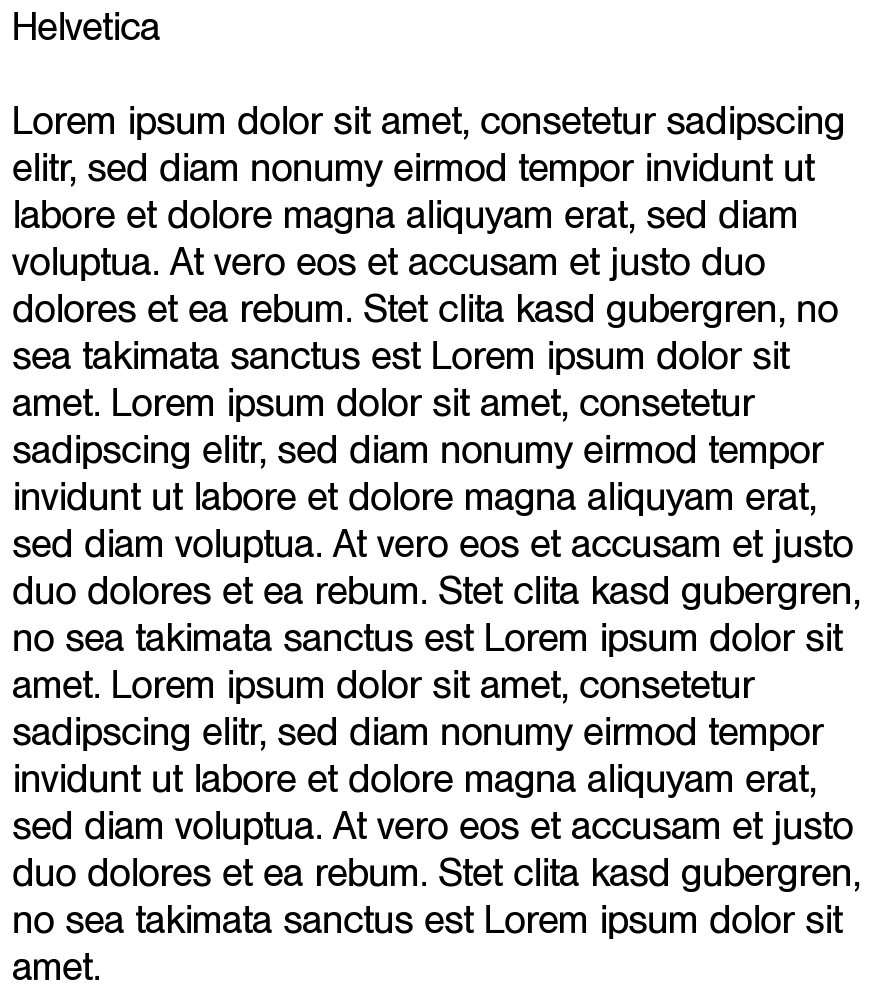
\includegraphics[width=.45\linewidth]{Lorem_Ipsum_Helvetica.png}
  \end{center}
  \caption{\label{fig:lorem} lorem ipsum rasterized plus a longish caption spanning two lines}
\end{figure}

Ut wisi enim ad minim veniam, quis nostrud exerci tation ullamcorper suscipit lobortis nisl ut aliquip ex ea commodo consequat. Duis autem vel eum iriure dolor in hendrerit in vulputate velit esse~\cite{Kindlmann1999}.

\subsection{Lorem}

\subsubsection{Ipsum}

\subsubsection{Dolor}

\begin{table}
\caption{
\label{tab:perf} lorem ipsum tabulated}
\centering
\vspace{0.3em}
\begin{tabular}{lrr}
dataset & full performance (fps) & half performance (ms)\\ \hline\\[-0.4em]
balls & 1,243 & 0.1 \\
buckets & 23 & 23 \\
bolts & 23,312,134.3 & 22.1 \\
\end{tabular}
\end{table}

\subsection{Lorem}


\subsection{Ipsum}

\subsection{Lorem}


\subsection{Ipsum}

\subsection{Lorem}


\subsection{Ipsum}


%% if specified like this the section will be ommitted in review mode
\acknowledgments{
We would like to thank our supervisors M. Krone and F. Fries(?) as well as our project examiner Prof. ... . We are grateful for the experience and knowledge that working on this project has given us.
This work was partially funded by cake and cookies.
}

\bibliographystyle{abbrv}
%%use following if all content of bibtex file should be shown
%\nocite{*}
\bibliography{template}
\end{document} 
